\documentclass[11pt,a4paper]{article}

\usepackage[T1]{fontenc}
\usepackage[utf8]{inputenc}
\usepackage[margin=25mm]{geometry}
\usepackage{amsmath,amssymb,bm}
\usepackage{booktabs}
\usepackage{array}
\usepackage{enumitem}
\usepackage{tikz}
\usetikzlibrary{arrows.meta,positioning,calc}
\usepackage[hidelinks]{hyperref}
\setlength{\emergencystretch}{3em}

\newcommand{\ud}{\,\mathrm{d}}

\title{\textbf{Electromagnetic--Acoustic Model of PWM-Excited\\
Differential Forces on a 120\,m Single-Core Cable Run}}
\author{Davide Bagnara}
\date{\today}

\begin{document}
\maketitle

\begin{abstract}
\noindent
This note extends the cable model of the companion document to the acoustic
domain. The audible emission observed near the converter cables is modeled as the
end of a four-stage chain: (i)~the differential PWM current ripple, (ii)~the
Amp\`ere forces it produces between the three single-core conductors, (iii)~the
transverse mechanical vibration of the cable spans, and (iv)~the acoustic
radiation of the vibrating conductors. The force is shown to be governed by the
\emph{differential} (positive/negative-sequence) currents, not the common mode,
confirming the field observation. The model reproduces the qualitative evidence:
a tonal line at the switching frequency, its conversion to a broadband
``flowing-water'' sound under random PWM, and the presence of emission on the
$120\ \mathrm{m}$ section while the $40\ \mathrm{m}$ section is silent. The
electrical parameters of the companion document are retained unchanged.
\end{abstract}

\tableofcontents
\bigskip

%======================================================================
\section{Scope and physical hypothesis}
%======================================================================
The site evidence is the following:
\begin{enumerate}[leftmargin=*,nosep]
\item the sound tracks the inverter PWM; with random (spread-spectrum) PWM the
tonal structure disappears and the emission becomes broadband, perceptually like
flowing water;
\item the $120\ \mathrm{m}$ cable section emits, the $40\ \mathrm{m}$ section does
not;
\item a tonal line coincides with the fixed converter switching frequency.
\end{enumerate}
The working hypothesis, examined and confirmed below, is that the excitation is the
\emph{differential} PWM current ripple acting through inter-conductor Amp\`ere
forces, and that the length dependence arises from the mechanical/acoustic
response, not from the electromagnetic source itself.

The arrangement modeled is three \emph{separate} single-core copper cables,
$90\ \mathrm{mm^2}$ each, length $\ell=120\ \mathrm{m}$. Separate single cores are
essential to the mechanism: unlike the bound conductors of a single three-core
cable, each single core is mechanically free to vibrate between its supports, so
the inter-conductor force does work on a movable structure. The per-unit-length
electrical parameters are taken unchanged from the companion document
(in particular $C_g=36\ \mathrm{nF}$ retained as requested, although the
common-mode capacitance does not enter the force).

\begin{figure}[h]
\centering
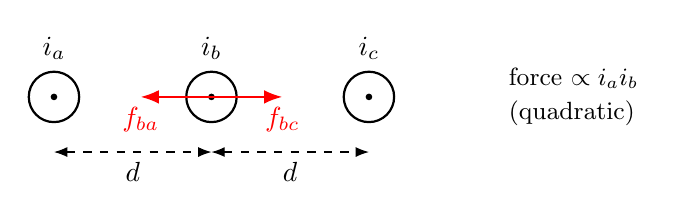
\begin{tikzpicture}[>=Latex]
\def\R{0.32}
\coordinate (A) at (-2.0,0);
\coordinate (B) at (0,0);
\coordinate (C) at (2.0,0);
\foreach \p/\n in {A/$i_a$,B/$i_b$,C/$i_c$}{
  \draw[thick] (\p) circle (\R);
  \fill (\p) circle (1.2pt);
}
\node at (-2.0,0.62) {$i_a$};
\node at (0,0.62) {$i_b$};
\node at (2.0,0.62) {$i_c$};
% forces on b
\draw[->,thick,red] (B) -- ($(B)+(-0.9,0)$) node[below]{$f_{ba}$};
\draw[->,thick,red] (B) -- ($(B)+(0.9,0)$) node[below]{$f_{bc}$};
\draw[<->,dashed] (-2.0,-0.7) -- (0,-0.7) node[midway,below]{$d$};
\draw[<->,dashed] (0,-0.7) -- (2.0,-0.7) node[midway,below]{$d$};
\node[align=left] at (4.6,0) {\small force $\propto i_a i_b$\\ \small (quadratic)};
\end{tikzpicture}
\caption{Transverse Amp\`ere forces on a single core from its two neighbors. The
force on each conductor is the vector sum of two contributions, each proportional
to the product of conductor currents.}
\label{fig:forces}
\end{figure}

%======================================================================
\section{From currents to forces}
%======================================================================
Two long parallel conductors $j,k$ at separation $d_{jk}$, carrying currents
$i_j,i_k$, exert on each other the transverse force per unit length
\begin{equation}
f_{jk}(t)=\frac{\mu_0}{2\pi\,d_{jk}}\,i_j(t)\,i_k(t),
\label{eq:ampere}
\end{equation}
attractive for like signs. This is the same magnetostatic law used for
short-circuit force calculations (IEC~60865). The net transverse force per unit
length on conductor $a$ is the vector sum from its neighbors,
\begin{equation}
\bm{f}_a(t)=\frac{\mu_0}{2\pi}\left[
\frac{i_a i_b}{d_{ab}}\,\hat{\bm{u}}_{ab}
+\frac{i_a i_c}{d_{ac}}\,\hat{\bm{u}}_{ac}\right],
\label{eq:fnet}
\end{equation}
with $\hat{\bm{u}}$ the unit vectors in the conductor cross-section
(Fig.~\ref{fig:forces}). The essential feature is the \emph{quadratic} dependence
on current: the force spectrum is the autocorrelation of the current spectrum, so
it contains sums and differences of all current frequency components.

%======================================================================
\section{Force spectrum and the dominance of the differential mode}
%======================================================================
Write each phase current as a fundamental term plus PWM ripple,
\begin{equation}
i_k(t)=\hat I_1\cos(\omega_1 t-\varphi_k)+\tilde\imath_k(t),
\qquad \varphi_k\in\{0,\tfrac{2\pi}{3},\tfrac{4\pi}{3}\},
\end{equation}
where $\tilde\imath_k$ has its spectral energy concentrated at the carrier
$f_{sw}$ and its multiples, with sidebands at $\pm m f_1$ (double-Fourier PWM
spectrum). Expanding the product in \eqref{eq:ampere},
\begin{equation}
i_a i_b=
\underbrace{\hat I_1^2\cos(\omega_1 t)\cos(\omega_1 t-\tfrac{2\pi}{3})}_{\text{(I) DC}+2f_1}
+\underbrace{\hat I_1\!\left[\cos(\omega_1 t)\,\tilde\imath_b+\cos(\omega_1 t-\tfrac{2\pi}{3})\,\tilde\imath_a\right]}_{\text{(II) fundamental}\times\text{ripple}}
+\underbrace{\tilde\imath_a\tilde\imath_b}_{\text{(III) ripple}^2}.
\label{eq:expand}
\end{equation}
The three groups give three force bands:
\begin{itemize}[leftmargin=*,nosep]
\item[(I)] a DC offset and a $2f_1$ component ($100\ \mathrm{Hz}$) --- the
classical conductor ``hum''. It is the largest in amplitude but radiates poorly
(see Sec.~\ref{sec:acou}) and lies below the perceptually critical band.
\item[(II)] components at $f_{sw}\pm m f_1$, i.e.\ \emph{centered on the switching
frequency}, of amplitude $\propto \hat I_1\,\hat{\tilde\imath}_{sw}$. This is the
audible tonal excitation.
\item[(III)] components at $2f_{sw}$, DC, and difference frequencies, of amplitude
$\propto \hat{\tilde\imath}_{sw}^2$, smaller because the ripple is small compared
with the fundamental.
\end{itemize}
The dominant audible force is therefore band~(II), whose amplitude per unit length
is
\begin{equation}
\boxed{\;\hat F_{sw}\approx\frac{\mu_0}{2\pi d}\,\hat I_1\,\hat{\tilde\imath}_{sw}\;}
\label{eq:Fsw}
\end{equation}
at frequency $\approx f_{sw}$ with $\pm f_1$ sidebands.

\paragraph{Differential vs.\ common mode.}
Equation~\eqref{eq:Fsw} settles the field intuition. The force is the product of a
\emph{large} differential fundamental current $\hat I_1$ (hundreds of amperes) and
the differential ripple $\hat{\tilde\imath}_{sw}$. The common-mode current is
small --- it is limited by the high common-mode impedance of the shield/earth loop
--- and, being squared or multiplied by itself in \eqref{eq:expand}, contributes a
force smaller by the ratio $(\hat I_{cm}/\hat I_1)^2$ or $(\hat I_{cm}/\hat I_1)$.
The audible mechanical excitation is thus governed by the positive/negative-sequence
(differential) currents; the common mode matters for the shield/EMC path of the
companion document, not for the acoustic force.

%======================================================================
\section{Coupling to the electrical cable model}
%======================================================================
The ripple amplitude $\hat{\tilde\imath}_{sw}$ entering \eqref{eq:Fsw} is set by the
volt-seconds the converter applies across the total per-phase series inductance
during a switching subinterval,
\begin{equation}
\hat{\tilde\imath}_{sw}\sim\frac{V_{dc}}{8\,L_\sigma\,f_{sw}},
\qquad L_\sigma=L_{\text{cable}}+L_{\text{load}},
\label{eq:ripple}
\end{equation}
plus any resonant amplification from the cable shunt capacitance. With the
companion-document value $L_{\text{cable}}=L_1'\ell=30\ \mu\mathrm{H}$ at
$120\ \mathrm{m}$ (and $10\ \mu\mathrm{H}$ at $40\ \mathrm{m}$), the cable
inductance is a minor addition to the motor leakage; the \emph{source} ripple is
nearly the same on both sections. The length dependence of the \emph{sound} must
therefore originate downstream, in the mechanical and acoustic response
(Secs.~\ref{sec:mech}--\ref{sec:length}), not in the electromagnetic forcing.

A secondary electrical effect is the differential resonance between $L_\sigma$ and
the cable capacitance $C_1=C_1'\ell$, at
$f_{0}=1/(2\pi\sqrt{L_\sigma C_1})$. For the reference values this lies in the tens
of kilohertz (well above $f_{sw}=3.8\ \mathrm{kHz}$) and is not the primary audible
mechanism, but it should be checked against the actual $L_\sigma$ because it scales
as $\ell^{-1/2}$ and moves downward with length.

%======================================================================
\section{Mechanical model of the cable span}\label{sec:mech}
%======================================================================
Each single core between two supports (cleats, span $L_s$) responds to the
distributed transverse force $f(z,t)$ as a beam under tension,
\begin{equation}
\rho_A\frac{\partial^2 w}{\partial t^2}
+EI\frac{\partial^4 w}{\partial z^4}
-T\frac{\partial^2 w}{\partial z^2}
=f(z,t),
\label{eq:beam}
\end{equation}
with $w$ the transverse displacement, $\rho_A$ the mass per unit length, $EI$ the
(low, because stranded) bending stiffness and $T$ the mechanical tension. The
undamped natural frequencies are, in the two limits,
\begin{equation}
\text{string: } f_n=\frac{n}{2L_s}\sqrt{\frac{T}{\rho_A}},
\qquad
\text{beam: } f_n=\frac{(\beta_n L_s)^2}{2\pi L_s^2}\sqrt{\frac{EI}{\rho_A}},
\label{eq:fn}
\end{equation}
with $\beta_nL_s=\{4.73,7.85,\dots\}$ for clamped ends. Resonant amplification of
the displacement occurs when a force harmonic $f_{sw}\pm m f_1$ coincides with an
$f_n$; the modal velocity at resonance is
\begin{equation}
\hat v_{\text{res}}\approx\frac{\hat F_{sw}}{\rho_A\,\omega_{sw}}\,Q,
\label{eq:vres}
\end{equation}
$Q$ being the mechanical quality factor of the span ($Q\!\sim\!10$--$50$ for a
lightly damped cleated conductor). Off resonance the same expression holds with
$Q\!\to\!1$.

\paragraph{Modal density.}
For a one-dimensional waveguide of total length $\ell$, the number of modes per
unit frequency scales with length,
\begin{equation}
\frac{\ud N}{\ud f}\propto \ell
\qquad\Longrightarrow\qquad
N_{120}\approx 3\,N_{40}.
\label{eq:moddensity}
\end{equation}
This is the key length-dependent quantity (Sec.~\ref{sec:length}).

%======================================================================
\section{Acoustic radiation}\label{sec:acou}
%======================================================================
A conductor of radius $a$ vibrating transversely is, acoustically, a line of
dipoles. The radiated sound power from a length $L$ is
\begin{equation}
W_{ac}=\rho_0 c\,\sigma_{\text{rad}}\,S\,\overline{v^2},
\qquad S=2\pi a L,\qquad \overline{v^2}=\tfrac12\hat v^2,
\label{eq:Wac}
\end{equation}
with $\rho_0 c=415\ \mathrm{Pa\,s/m}$ and $\sigma_{\text{rad}}$ the radiation
efficiency. For transverse (dipole) motion $\sigma_{\text{rad}}$ rises with the
compactness ratio $ka=2\pi f a/c$. At $f_{sw}=3.8\ \mathrm{kHz}$ and
$a=9\ \mathrm{mm}$, $ka\approx0.63$, giving an order-of-unity, moderately efficient
radiator ($\sigma_{\text{rad}}\sim0.2$); the $100\ \mathrm{Hz}$ hum, by contrast,
has $ka\approx0.017$ and is an extremely poor radiator, which is why the audible
emission is the switching tone and not the (larger) $100\ \mathrm{Hz}$ force. The
sound power level is $L_W=10\log_{10}(W_{ac}/10^{-12})\ \mathrm{dB}$.

%======================================================================
\section{Numerical estimate}\label{sec:numbers}
%======================================================================
Representative site values (to be replaced by measured data) are listed in
Table~\ref{tab:par}.

\begin{table}[h]
\centering
\caption{Representative parameters for the estimate.}
\label{tab:par}
\begin{tabular}{@{}lll@{}}
\toprule
Quantity & Symbol & Value \\
\midrule
Fundamental current (peak) & $\hat I_1$ & $283\ \mathrm{A}$ ($200\ \mathrm{A}$ rms) \\
Carrier-harmonic ripple (amp.) & $\hat{\tilde\imath}_{sw}$ & $20\ \mathrm{A}$ \\
Conductor separation & $d$ & $40\ \mathrm{mm}$ \\
Fundamental / switching freq. & $f_1,f_{sw}$ & $50\ \mathrm{Hz}$, $3.8\ \mathrm{kHz}$ \\
Cable mass per length & $\rho_A$ & $1.3\ \mathrm{kg/m}$ \\
Conductor outer radius & $a$ & $9\ \mathrm{mm}$ \\
Mechanical quality factor & $Q$ & $1$ (off-res.) / $30$ (res.) \\
Radiation efficiency & $\sigma_{\text{rad}}$ & $0.2$ \\
\bottomrule
\end{tabular}
\end{table}

\paragraph{Forces.}
From \eqref{eq:Fsw} and the $2f_1$ part of \eqref{eq:expand}, with
$\mu_0/(2\pi d)=5\times10^{-6}\ \mathrm{N/A^2}$:
\[
\hat F_{2f_1}=\frac{\mu_0}{2\pi d}\frac{\hat I_1^2}{2}=0.20\ \mathrm{N/m}
\quad(100\ \mathrm{Hz}),
\qquad
\hat F_{sw}=\frac{\mu_0}{2\pi d}\hat I_1\hat{\tilde\imath}_{sw}=0.028\ \mathrm{N/m}
\quad(\approx f_{sw}).
\]

\paragraph{Velocity.}
From \eqref{eq:vres}, $\hat v=0.9\ \mu\mathrm{m/s}$ off resonance ($Q=1$) and
$27\ \mu\mathrm{m/s}$ at resonance ($Q=30$).

\paragraph{Sound.}
From \eqref{eq:Wac}, Table~\ref{tab:spl} compares the two sections. The model
predicts an audible tone ($\sim 42\ \mathrm{dB}$ at $1\ \mathrm{m}$) on the
$120\ \mathrm{m}$ section when a span mode is excited, and an inaudible level
($\sim 8\ \mathrm{dB}$) on the non-resonant $40\ \mathrm{m}$ section.

\begin{table}[h]
\centering
\caption{Predicted radiated levels (SPL at $1\ \mathrm{m}$, point-source
approximation).}
\label{tab:spl}
\begin{tabular}{@{}lcccc@{}}
\toprule
Section & State & $\hat v$ & $L_W$ & SPL@1\,m \\
\midrule
$120\ \mathrm{m}$ & resonant ($Q{=}30$)    & $27\ \mu\mathrm{m/s}$  & $53\ \mathrm{dB}$ & $\approx 42\ \mathrm{dB}$ \\
$40\ \mathrm{m}$  & off-resonance ($Q{=}1$)& $0.9\ \mu\mathrm{m/s}$ & $19\ \mathrm{dB}$ & $\approx 8\ \mathrm{dB}$ \\
$40\ \mathrm{m}$  & (if resonant)          & $27\ \mu\mathrm{m/s}$  & $49\ \mathrm{dB}$ & $\approx 38\ \mathrm{dB}$ \\
\bottomrule
\end{tabular}
\end{table}

%======================================================================
\section{Explanation of the field observations}\label{sec:length}
%======================================================================
\paragraph{Why $120\ \mathrm{m}$ emits and $40\ \mathrm{m}$ is silent.}
The per-unit-length force is the same on both sections (same currents, separation
and carrier). Three length-dependent factors act downstream:
\begin{enumerate}[leftmargin=*,nosep]
\item \textbf{Modal coincidence (dominant).} By \eqref{eq:moddensity} the long run
has three times the modal density. Under \emph{fixed} (narrow-band) PWM the tonal
force is far more likely to coincide with a lightly damped span mode of the
$120\ \mathrm{m}$ run; the sparser modes of the $40\ \mathrm{m}$ run can fall in a
gap, leaving it near the off-resonance level. The resonant/non-resonant contrast
in Table~\ref{tab:spl} is a $34\ \mathrm{dB}$ difference.
\item \textbf{Radiating area.} For equal surface velocity the longer cable radiates
$\,10\log_{10}(120/40)\approx4.8\ \mathrm{dB}$ more.
\item \textbf{Installation/damping.} Longer free spans or lower clamping damping on
the $120\ \mathrm{m}$ run lower $f_n$ and raise $Q$, both increasing emission.
\end{enumerate}

\paragraph{Why random PWM gives a ``water'' sound.}
Random/spread-spectrum PWM replaces the discrete carrier line with a broadband
spectrum. By \eqref{eq:expand}, band~(II) of the force is correspondingly spread
across frequency, so instead of driving one resonant mode it distributes energy
over many modes at low spectral density. The radiated field loses its tonal
character and becomes broadband noise --- perceptually the observed flowing-water
sound --- and, crucially, the peak modal excitation drops, which is the same
mechanism by which random PWM is used to reduce acoustic noise in drives.

%======================================================================
\section{Confirmation and mitigation}
%======================================================================
\paragraph{To confirm the model.}
\begin{itemize}[leftmargin=*,nosep]
\item Measure the acoustic spectrum and check the tonal line moves with $f_{sw}$
and its sidebands sit at $f_{sw}\pm m f_1$.
\item A simple bump/impact test on a $120\ \mathrm{m}$ span identifies the span
natural frequencies; coincidence of one $f_n$ with $f_{sw}\pm m f_1$ confirms the
mechanism.
\item Verify the level scales with $\hat I_1\,\hat{\tilde\imath}_{sw}$ (load and
$f_{sw}$ dependence) as predicted by \eqref{eq:Fsw}.
\end{itemize}

\paragraph{Mitigation levers (from the model).}
\begin{itemize}[leftmargin=*,nosep]
\item Move $f_{sw}$ off the coincident span mode, or adopt random/spread-spectrum
PWM (spreads band~(II); lowers peak excitation).
\item Detune the mechanical resonance: change cleat spacing $L_s$ (shifts $f_n$ in
\eqref{eq:fn}) or add damped clamps (raises losses, lowers $Q$).
\item Reduce the force: increase conductor separation $d$ (\eqref{eq:Fsw} scales as
$1/d$), or reduce $\hat{\tilde\imath}_{sw}$ with a higher $f_{sw}$ or an output
$\mathrm{d}v/\mathrm{d}t$/sine filter.
\end{itemize}

%======================================================================
\section*{References}
\addcontentsline{toc}{section}{References}
%======================================================================
\begin{thebibliography}{99}

\bibitem{holmes} D.~G.~Holmes and T.~A.~Lipo, \emph{Pulse Width Modulation for
Power Converters: Principles and Practice}. Hoboken, NJ: Wiley--IEEE Press, 2003.

\bibitem{habetler} T.~G.~Habetler and D.~M.~Divan, ``Acoustic noise reduction in
sinusoidal PWM drives using a randomly modulated carrier,'' \emph{IEEE Trans. Power
Electron.}, vol.~6, no.~3, pp.~356--363, Jul.~1991.

\bibitem{iec60865} \emph{Short-Circuit Currents --- Calculation of Effects ---
Part~1: Definitions and Calculation Methods}, IEC~60865-1, 2011.

\bibitem{paul} C.~R.~Paul, \emph{Analysis of Multiconductor Transmission Lines},
2nd ed. Hoboken, NJ: Wiley--IEEE Press, 2008.

\bibitem{fahy} F.~Fahy and P.~Gardonio, \emph{Sound and Structural Vibration:
Radiation, Transmission and Response}, 2nd ed. Oxford, U.K.: Academic Press, 2007.

\bibitem{junger} M.~C.~Junger and D.~Feit, \emph{Sound, Structures, and Their
Interaction}, 2nd ed. Cambridge, MA: MIT Press, 1986.

\bibitem{cremer} L.~Cremer, M.~Heckl, and B.~A.~T.~Petersson,
\emph{Structure-Borne Sound}, 3rd ed. Berlin, Germany: Springer, 2005.

\bibitem{vonjouanne} A.~von Jouanne and P.~N.~Enjeti, ``Design considerations for
an inverter output filter to mitigate the effects of long motor leads in ASD
applications,'' \emph{IEEE Trans. Ind. Appl.}, vol.~33, no.~5, pp.~1138--1145,
Sep./Oct.~1997.

\end{thebibliography}

%======================================================================
\appendix
\section{Signal chain}
%======================================================================
\begin{center}
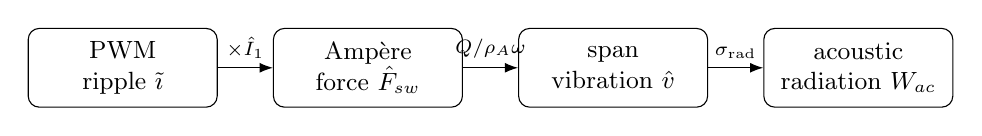
\begin{tikzpicture}[>=Latex,node distance=4mm and 7mm,
  block/.style={draw,rounded corners,minimum height=10mm,minimum width=24mm,align=center,font=\small}]
\node[block] (a) {PWM\\ripple $\tilde\imath$};
\node[block,right=of a] (b) {Amp\`ere\\force $\hat F_{sw}$};
\node[block,right=of b] (c) {span\\vibration $\hat v$};
\node[block,right=of c] (d) {acoustic\\radiation $W_{ac}$};
\draw[->] (a)--(b) node[midway,above,font=\scriptsize]{$\times\hat I_1$};
\draw[->] (b)--(c) node[midway,above,font=\scriptsize]{$Q/\rho_A\omega$};
\draw[->] (c)--(d) node[midway,above,font=\scriptsize]{$\sigma_{\text{rad}}$};
\end{tikzpicture}
\end{center}
\noindent
The four transfer factors are: the differential fundamental current $\hat I_1$
(force generation, Eq.~\eqref{eq:Fsw}); the mechanical mobility $Q/(\rho_A\omega)$
(Eq.~\eqref{eq:vres}); and the radiation efficiency $\sigma_{\text{rad}}$
(Eq.~\eqref{eq:Wac}). The length $\ell$ enters through the modal density
\eqref{eq:moddensity} (probability of resonance) and the radiating area
\eqref{eq:Wac}.

\end{document}
